\documentclass[../../main]{subfiles}

\begin{document}
\subsection[Evolution of AGV Mechanical Systems]{Evolution of AGV Mechanical Systems: Key Innovations and Applications}

% Automated Guided Vehicles (AGVs) represent a significant advancement in
% material handling automation. Research in this field focuses on
% improving navigation systems, obstacle avoidance, fleet management, and
% system integration capabilities. Modern AGVs incorporate advanced
% technologies like AI and sophisticated sensors to enhance their
% autonomous operation and decision-making abilities.
% \newpage

% \subsection{Previous Studies on AGV Mechanical Design}

Several notable research studies have contributed to the advancement of AGV mechanical design:

In a 2020 study, Ze Cui and Saishuai Huang developed an innovative Automated Guided Vehicle (AGV) system for hospital medicine transportation. The system features a comprehensive mechanical structure comprising an AGV chassis, scissor lifting mechanism, rotary platform, extension mechanism, and vacuum sucker actuator. The control system utilizes Robot Operating System with magnetic stripe navigation and RFID site labels, while incorporating safety features such as ultrasonic sensors and LiDAR. Through experimental testing, this hospital-focused system, designed specifically for transporting medicine boxes between warehouses and department stations, successfully demonstrated its ability to meet all design requirements and perform its intended functions effectively.

In another 2020 study, Taher Deemyad, Anish Sebastian, and Ryan Moeller focused on the chassis design and analysis of an AGV specifically designed for agricultural applications. Their research centered on developing a four-wheel powered vehicle for identifying and removing potatoes affected by virus Y (PVY) in the field. The challenging nature of potato fields, with their rough terrain and deep irrigation ruts, necessitated a robust chassis design. The team employed optimization routines to determine ideal chassis dimensions and materials, conducting seven different stress analyses to refine the design. Their prototype successfully passed all design requirements in CAD modeling (SolidWorks) and was subsequently built and field-tested, demonstrating the effectiveness of their analytical approach to AGV chassis design.

In a 2024 study by researchers from the \textit{International Journal for Research in Applied Science \& Engineering Technology (IJRASET)}, a multipurpose scissor lift mechanism was developed for various industrial applications. The study focused on creating a cost-effective and efficient lifting solution that could be used in garages, manufacturing facilities, and construction sites. The design incorporated a hydraulic system for power transmission and featured a robust scissor mechanism capable of lifting loads up to 500kg. The researchers conducted comprehensive structural analysis using CAD software to validate the design's safety and stability. Their experimental results demonstrated the lift's reliability and versatility across different operating conditions, while maintaining a focus on operator safety and ease of maintenance.

These research contributions have significantly influenced modern AGV mechanical design, leading to more efficient, reliable, and adaptable systems suitable for various industrial applications.


\subsection{Research Gaps and Justification}
Despite significant advancements in AGV mechanical design, several
research gaps remain to be addressed:

\begin{enumerate}
\item
  Limited research exists on AGV adaptation to dynamic industrial
  environments where layout changes are frequent. Most existing studies
  focus on static or semi-static environments.
\item
  There is insufficient investigation into energy optimization for
  heavy-load AGVs, particularly in continuous operation scenarios.
\item
  The integration of predictive maintenance systems with mechanical
  design aspects remains understudied, creating opportunities for
  further research.
\item
  Current literature lacks comprehensive studies on mechanical design
  solutions for multi-terrain AGV applications, particularly in hybrid
  indoor-outdoor environments.
\item
  There is a notable gap in research regarding standardization of
  mechanical interfaces for modular AGV components, which could enhance
  maintenance and upgradeability.
\end{enumerate}

These identified gaps justify the need for further research in AGV
mechanical design, particularly focusing on adaptability, energy
efficiency, and system integration. This study aims to address several
of these gaps by proposing novel solutions in AGV mechanical design.

These identified gaps justify the need for further research in AGV mechanical design, particularly focusing on adaptability, energy efficiency, and system integration. This study aims to address several of these gaps by proposing novel solutions in AGV mechanical design.

The literature review has highlighted the evolution of AGV mechanical
design, from fundamental navigation and chassis developments to modern
innovations in materials and smart technologies. While significant
advancements have been made in areas such as flexible navigation,
optimized chassis design, drive systems, and payload handling
mechanisms, several research gaps remain. These include the need for
better adaptation to dynamic environments, improved energy optimization
for heavy loads, integration of predictive maintenance, multi-terrain
capabilities, and standardization of modular components. These
identified gaps provide the foundation for further research in AGV
mechanical design.
% \newpage
% \subsection{Physical Design Constraints} %realistic constrait

% The design and construction of a single-level scissor lift AGV with
% chassis frame structure must consider several practical constraints:



% The load capacity constraints require that the maximum payload capacity is clearly defined and maintained within safety limits. Additionally, the weight distribution across the chassis frame must be balanced to avoid causing structural stress. It is also important to take into account the material strength limitations of the frame components.

% \subsubsection{Load Capacity Constraints}

% Maximum payload capacity must be clearly defined and maintained within safety limits. Weight distribution across the chassis frame must be balanced to prevent structural stress. Material strength limitations of frame components must be considered.


% \subsubsection{Dimensional Constraints}

% The dimensional constraints include overall height limitations in both collapsed and extended positions, as well as a maximum allowable footprint based on operational space requirements. Additionally, there are minimum ground clearance requirements for safe operation, and turning radius limitations must be considered based on the operational environment.

% \subsubsection{Material and Manufacturing Constraints}

% The material and manufacturing constraints include considerations for material availability and cost, as well as limitations imposed by manufacturing capabilities and tooling. Additionally, welding and assembly requirements must be taken into account, along with constraints related to surface treatment and finishing.

% \subsection{Operational Constraints}

% \subsubsection{Safety Requirements}

% Compliance with safety standards and regulations is critical to avoid legal issues and ensure user safety. The implementation of emergency stop mechanisms must be robust, easily accessible, and tested under various operational scenarios. Stability requirements during movement and lifting operations should account for dynamic loads, environmental conditions, and potential human errors. Additionally, safety factor considerations in structural design must include material strength, fatigue resistance, and redundancy to prevent catastrophic failures.
% \newpage
% \subsubsection{Performance Constraints}

% The system must adhere to maximum lifting speed limitations to ensure safe and controlled operations. Operational cycle time requirements should be optimized to balance efficiency and safety while avoiding unnecessary strain on components. Power consumption limitations are critical to minimize energy usage and align with sustainability goals. Additionally, maintenance accessibility requirements must be integrated into the design to facilitate ease of upkeep and reduce downtime.

% \subsubsection{Environmental Constraints}

% The system must operate within specified temperature range limitations to ensure reliable performance under varying environmental conditions. Considerations for humidity and moisture exposure are essential to prevent corrosion and electrical failures. The design should account for floor surface conditions and variations to maintain stability and safety during operations. Additionally, limitations related to dust and debris exposure must be addressed to protect sensitive components and ensure long-term functionality.

% \subsection{Economic Constraints} %no usefull content

% The development and implementation of the AGV system must consider
% various economic factors:

% \begin{itemize}
% \item
%   Budget limitations for materials and components
% \item
%   Manufacturing cost constraints
% \item
%   Maintenance cost considerations
% \item
%   Return on investment requirements
% \end{itemize}

% \subsection{Integration Constraints} % no usefull content

% The AGV system must be designed considering integration with existing
% systems and infrastructure:

% \begin{itemize}
% \item
%   Compatibility with existing facility layout
% \item
%   Integration with control systems and software
% \item
%   Interface requirements with other equipment
% \item
%   Future upgrade and modification possibilities
% \end{itemize}
\subsection{METHOD OF AGV DESIGN}
\begin{figure}[ht]
  \centering
  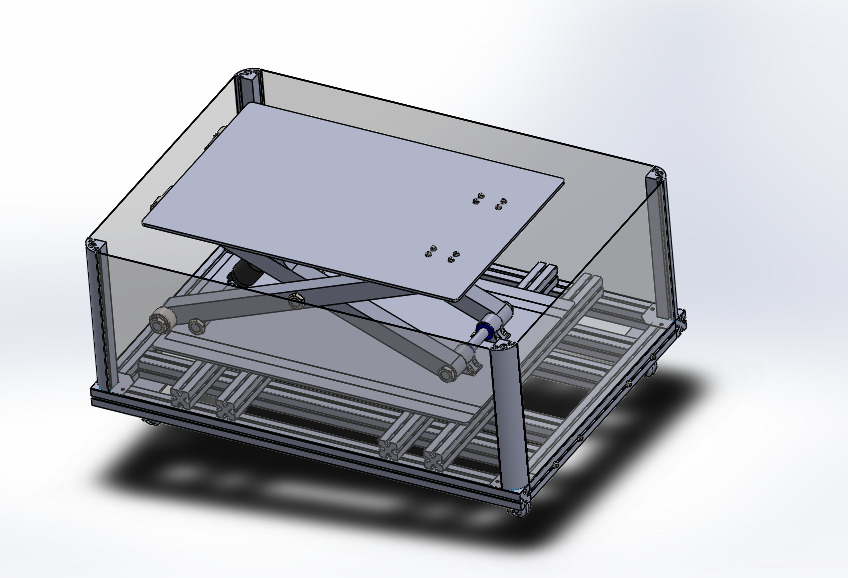
\includegraphics[width=0.6\textwidth]{img/image1.jpg}
  \caption{AGV Design Process}
\end{figure}

\subsubsection{Single level Scissor lift design}

The single level scissor lift mechanism is a crucial component of the
AGV design,\\ enabling vertical movement of loads through mechanical
advantage. This section details the design parameters and specifications
of the scissor lift system, which was carefully\\ engineered to meet the
required load capacity and operational requirements.\\The mechanism
consists of interconnected arms that form an
\textquotesingle X\textquotesingle{} pattern, allowing for smooth
vertical extension and retraction.

The design incorporates various dimensional parameters and mechanical
elements that work together to achieve efficient lifting operation. Key
considerations include the nominal load capacity, platform weights, and
critical arm dimensions that determine the lift\textquotesingle s range
of motion and stability.

\begin{figure}[h]
\centering
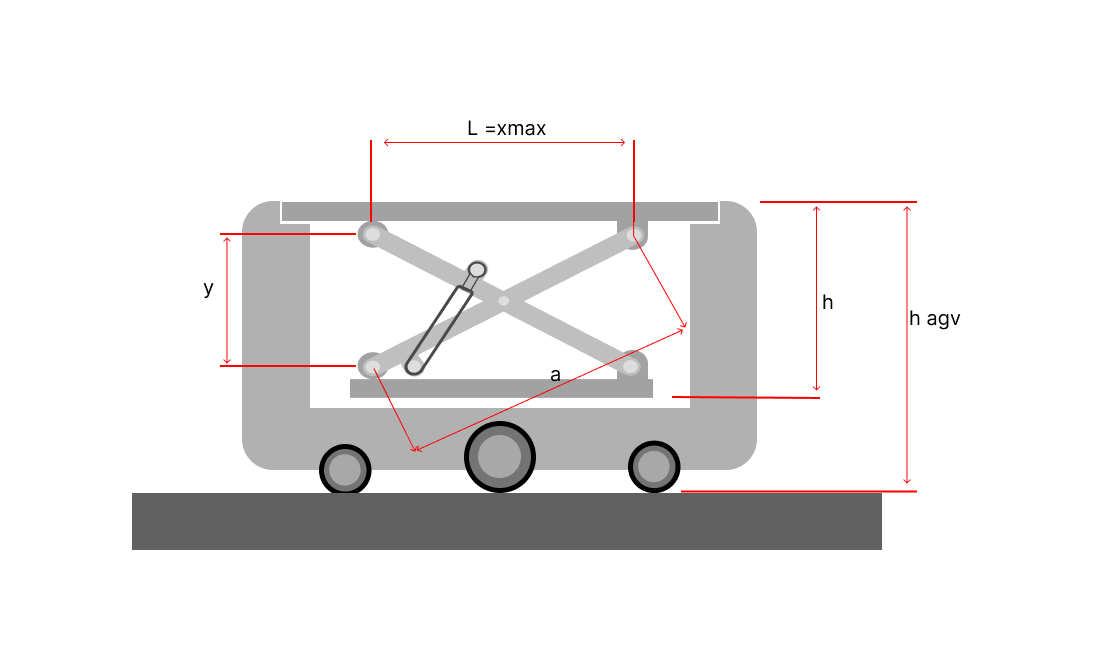
\includegraphics[width=0.5\textwidth]{img/image003.png}
\caption{Single level scissor lift in an Automated Guidance Vehicle}
\end{figure}
\newpage
The parameters listed in the table above were carefully chosen based on
several key design considerations for the AGV system:

\begin{enumerate}
\def\labelenumi{\arabic{enumi}.}
\item
  Load Capacity: The nominal load (F) of 1.22625 kN was selected to
  accommodate standard industrial pallets and containers while
  maintaining a safety margin. This capacity allows the AGV to handle
  typical warehouse loads efficiently.
\item
  Platform Dimensions: The upper platform weight (m1) of 22.6 kg
  represents an optimized balance between structural integrity and
  overall system weight. The scissor lift arms\textquotesingle{} weight
  ($m^2$) of 3.724 kg was achieved through material selection and
  structural optimization to minimize power requirements while
  maintaining stability.
\item
  Operational Range: The maximum distance between articulations (L = 0.6
  m) was determined based on the required lifting height and the
  available space constraints on the AGV chassis. This dimension, along
  with the arm lengths (a = 0.6466 m), enables the desired vertical
  travel range while maintaining a compact footprint.
\item
  Mechanical Stability: The arm dimensions (b, c, d, e) were calculated
  to provide optimal mechanical advantage and structural stability
  throughout the lifting range. These dimensions ensure smooth operation
  and minimize stress concentrations at the pivot points.
\item
  System Configuration: The use of two pairs of arms ($n_1$ = 2) and a
  single hydraulic cylinder ($n_2$ = 1) represents an efficient design that
  balances complexity, cost, and reliability. This configuration
  provides adequate support and lifting capability while minimizing the
  number of moving parts and potential failure points.
\end{enumerate}

These parameters work together to create a scissor lift mechanism that
meets the AGV\textquotesingle s requirements for load capacity,
stability, and operational efficiency while maintaining a compact form
factor suitable for automated warehouse operations.
\newpage
\renewcommand{\arraystretch}{1.4} % Increase row height for better readability
\begin{table}[h!]
  \centering
  \begin{tcolorbox}[
    colback=red!5!white,colframe=red!75!black,
    title={\textbf{Parameters}},
    fonttitle=\bfseries, coltitle=white, width=\linewidth
]
  \begin{adjustbox}{max width=\linewidth} % Ensures the table fits within the page
  \begin{tabular}{|c|c|p{0.75\linewidth}|}
  \hline\rowcolor{red!20}
  \textbf{Parameter} & \textbf{Value} & \textbf{Description} \\ \hline
  $F$ & $1.22625 \, \text{kN}$ & Nominal load \\ \hline
  $m_1$ & $22.6 \, \text{kg}$ & Upper platform weight \\ \hline
  $m_2$ & $3.724 \, \text{kg}$ & Weight of scissors lift arms \\ \hline
  $L$ & $0.6 \, \text{m}$ & Maximum distance between "1" and "2" articulations \\ \hline
  $l$ & $0.3 \, \text{m}$ & $L/2$ \\ \hline
  $h_1 = h_2$ & $0.006 \, \text{m}$ & Height of upper and lower platforms \\ \hline
  $y$ & $0.241 \, \text{m}$ & Height of the scissor mechanism without the platforms \\ \hline
  $a$ & $0.6466 \, \text{m}$ & Arm dimension \\ \hline
  $b$ & $0.230 \, \text{m}$ & Arm dimension \\ \hline
  $c$ & $0.06466 \, \text{m}$ & Arm dimension \\ \hline
  $d$ & $0.055 \, \text{m}$ & Arm dimension \\ \hline
  $e$ & $0.027275 \, \text{m}$ & Arm dimension \\ \hline
  $n_1$ & $2$ & Number of pairs of arms forming the mechanism \\ \hline
  $n_2$ & $1$ & Number of hydraulic cylinders used for scissors lift actuation \\ \hline
  \end{tabular}
\end{adjustbox}
\end{tcolorbox}
\caption{Parameters and their descriptions}
  \end{table}

  \subparagraph{Note:} 
  L/2 (0.3 m) represents the upper platform middle point. The
  value "L" (0.6 m) is specifically used for locating the center of
  gravity (CoG) of the upper platform weight ($m_1$). According to the
  design parameters, L is less than the arm length $a$ (0.6466 m).

\begin{figure}[h]
\centering
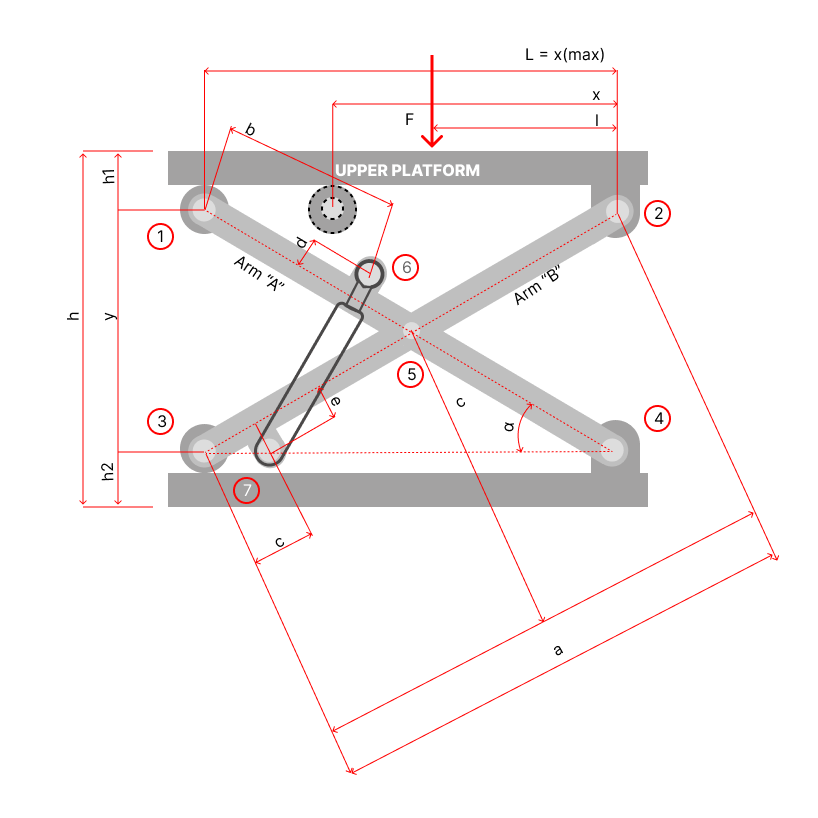
\includegraphics[width=0.8\textwidth]{img/image005.png}
\caption{Single level Scissor lift dimensions}
\end{figure}
\newpage
\subsection{Load analysis}\label{load-analysis}

Maximum load analysis:

The maximum load analysis is crucial for ensuring the safe and reliable
operation of the scissor lift mechanism. This analysis considers various
forces acting on the system when it is loaded to its maximum capacity.
The following factors are evaluated:

\begin{itemize}
\item
  Static load distribution across the lifting mechanism
\item
  Dynamic forces during lifting and lowering operations
\item
  Stress concentrations at critical points
\item
  Safety factors and load limits
\end{itemize}

The analysis takes into account both the nominal load (F) of 1.22625 kN
and the self-weight of the system components, including the upper
platform weight (m1) and the scissors lift arms weight (m2). This
comprehensive evaluation ensures that all structural elements are
adequately designed to handle the maximum expected loads while
maintaining a suitable safety margin.

\subsubsection{Load distribution:}
The load distribution can be mathematically expressed through the
following relationships:\\
For a load F applied at distance l from point 1, the distribution
coefficients q and r are determined by:
\begin{description}
  \item[Moment equation about point 1:]
    \begin{equation}
      F(q)(r) = F(l)
    \end{equation}
  
  \item[Roller support coefficient:]
    \begin{equation}
      q = \frac{l}{x}
    \end{equation}
    where $x$ is the distance between supports, and $q$ represents the roller support coefficient.
  
  \item[Moment equation about point 2:]
    \begin{equation}
      F(r)(x) = F(x-l)
    \end{equation}
  
  \item[Complementary relationship between coefficients:]
    \begin{equation}
      r = 1 - \frac{l}{x} = 1 - q
    \end{equation}
  \end{description}


These equations demonstrate that:
\begin{itemize}
\item
  The load distribution is directly proportional to the distance ratios
\item
  As x changes during the lifting operation, both q and r adjust
  accordingly
\item
  The sum of coefficients always equals 1, maintaining equilibrium
\end{itemize}
\begin{figure}[ht]
  \centering
  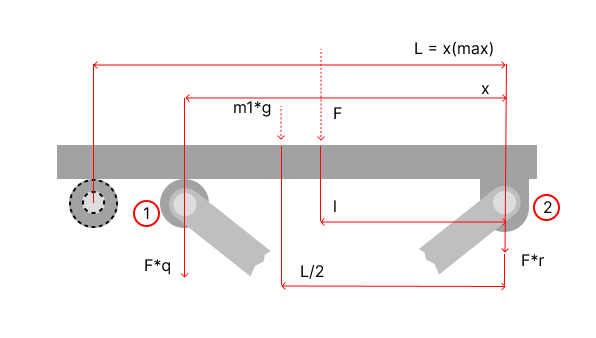
\includegraphics[width=0.3159\textwidth]{img/image015.png}
  \caption{load distribution coefficients at point 1 and
  2}
\end{figure}
\newpage

\subsubsection{Dead load}

The dead load refers to the permanent, static weight of the scissor lift
mechanism\textquotesingle s structural components. This includes all
fixed elements that contribute to the overall weight of the system,
regardless of the operational state.

The weight and load acting on the scissor lift mechanism itself consists
of the following components:

\begin{table}[h!]
  \centering
  \begin{tcolorbox}[
    colback=red!5!white,colframe=red!75!black,
    title={\textbf{Component Details and Weights}},
    fonttitle=\bfseries, coltitle=white, width=\linewidth
]
  \begin{tabular}{|l|c|p{6cm}|r|}
    \hline \rowcolor{red!20}
    \textbf{Component} & \textbf{Quantity} & \textbf{Description} & \textbf{(kg)} \\ \hline
    Plates (upper and lower) & 2 & Primary support platforms & 22.6 \\ \hline
    Scissor arms & 4 & Main lifting mechanism components & 5.08 \\ \hline
    Bearings & 4 & Facilitates smooth movement at pivot points & 1.0 \\ \hline
    Pin supports & 4 & Structural connection points & 0.48 \\ \hline
    Actuator cylinder & 1 & Hydraulic lifting mechanism & 3.5 \\ \hline
    Shafts (varying length) & 6 & Mechanical linkage components & 2.4 \\ \hline
    Fasteners & Multiple & Bolts and nuts for assembly & 0.5 \\ \hline
    \multicolumn{3}{|l|}{\textbf{Dead weight}} & \textbf{35.56} \\ \hline
  \end{tabular}
\end{tcolorbox}
\caption{Component Details and Weights}
  \end{table}


The dead load must be carefully considered in the overall system design
as it:

\begin{itemize}
\item
  Affects the power requirements of the lifting mechanism
\item
  Influences the selection of structural materials
\item
  Impacts the overall energy efficiency of the system
\item
  Contributes to the total load that must be supported by the AGV
  chassis
\end{itemize}
\newpage
\subsubsection{Forces on the lift}

The forces acting on the scissor lift mechanism can be analyzed through
a series of mathematical equations that describe the relationship
between various components. These equations account for both static and
dynamic forces during operation:

\begin{figure}[ht]
\centering
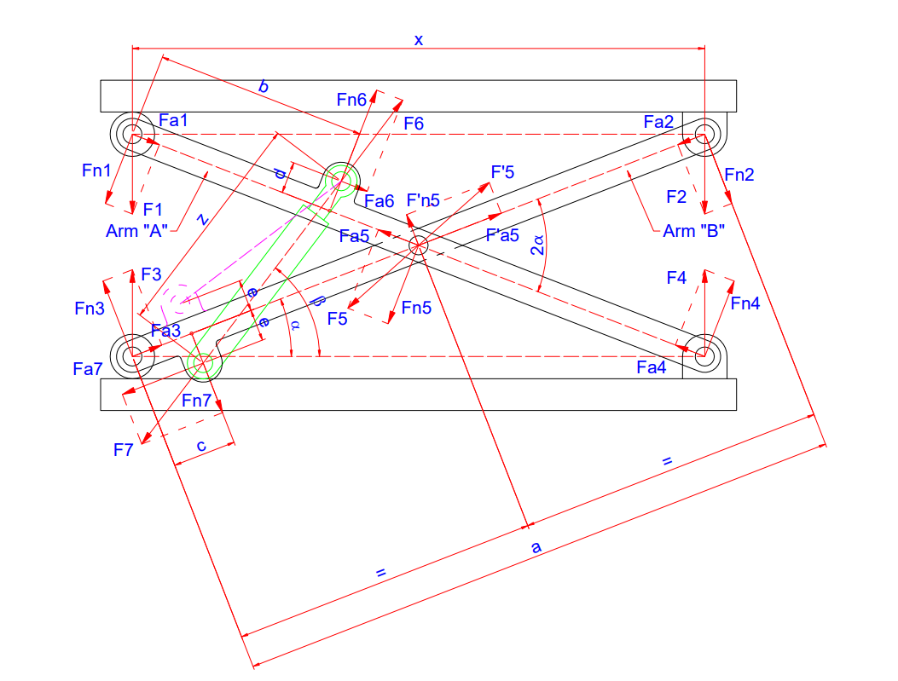
\includegraphics[width=0.7\textwidth]{img/image017.png}
\caption{Forces acting on the scissor lift}
\end{figure}

For a given angle $\alpha$, the following forces are calculated:

\begin{itemize}
\item
  F1 to F4: Primary forces acting on the scissor arms
\item
  Fn1 to Fn4: Normal force components
\item
  Fa1 to Fa4: Axial force components
\item
  F6 and F7: Forces in the hydraulic cylinder arrangement
\end{itemize}

The analysis is divided into two main sections:

Arm "A" Analysis

The forces on Arm "A" are calculated considering moments around point 5,
with the following key equations:

\begin{equation}
  F_{n1}\left(\frac{a}{2}\right) + F_{n4}\left(\frac{a}{2}\right) - F_{n6}\left(\frac{a}{2} - b\right) - F_{a6}(d) = 0
  \end{equation}
  \begin{equation}
    F_6 = \left(F_{n1} \frac{a}{2} + F_{n4} \frac{a}{2}\right) \left[\cos(90^\circ - \alpha - \beta)\left(\frac{a}{2} - b\right) + \sin(90^\circ - \alpha - \beta)d\right]
    \end{equation}
    \begin{equation}
      F_5 = \sqrt{{F_{n5}}^2 + {F_{a5}}^2}
  \end{equation}

  Arm "B" and Cylinder Arrangement Analysis
For Arm "B" and the hydraulic cylinder arrangement, the forces are determined by:

\begin{equation}
  F_{n2}\left(\frac{a}{2}\right) + F_{n3}\left(\frac{a}{2}\right) - F_{n7}\left(\frac{a}{2} - c\right) - F_{a7}(e) = 0
\end{equation}
\begin{equation}
  F_7 = \left(F_{n2}\frac{a}{2} + F_{n3}\frac{a}{2}\right) \left[\sin(\beta - \alpha)\frac{a}{2} - c - \cos(\beta - \alpha)e\right]
\end{equation}


These equations form the basis for understanding the force distribution
throughout the scissor lift mechanism and are essential for ensuring
proper design and operation of the system.

The following table shows the calculated forces at different angles ($\alpha$)
of the scissor lift mechanism:

\begin{table}[h!]
    \centering
    \begin{tcolorbox}[
      colback=red!5!white,colframe=red!75!black,
      title={\textbf{Forces}},
      fonttitle=\bfseries, coltitle=white, width=\linewidth]
    \begin{tabular}{|c|c|c|c|c|c|c|c|}
        \hline \rowcolor{red!20}
        $\alpha$ (degrees) & $F_1$ (kN) & $F_2$ (kN) & $F_3$ (kN) & $F_4$ (kN) & $F_5$ (kN) & $F_6$ (kN) & $F_7$ (kN) \\ \hline
        22 & 2.84 & 2.76 & 2.76 & 2.84 & 3.12 & 4.28 & 4.18 \\ \hline
        24 & 2.92 & 2.83 & 2.83 & 2.92 & 3.24 & 4.42 & 4.32 \\ \hline
        26 & 3.01 & 2.91 & 2.91 & 3.01 & 3.38 & 4.58 & 4.48 \\ \hline
        28 & 3.12 & 3.02 & 3.02 & 3.12 & 3.54 & 4.76 & 4.66 \\ \hline
        30 & 3.24 & 3.14 & 3.14 & 3.24 & 3.72 & 4.96 & 4.86 \\ \hline
        32 & 3.38 & 3.28 & 3.28 & 3.38 & 3.92 & 5.18 & 5.08 \\ \hline
    \end{tabular}
  \end{tcolorbox}
    \caption{Forces acting on scissor lift components at various angles of operation}
\end{table}

Where:

\begin{itemize}
\item
  F1 to F4 represent the primary forces on the scissor arms
\item
  F5 is the resultant force at the central pivot point
\item
  F6 and F7 are the forces in the hydraulic cylinder arrangement
\end{itemize}
The table demonstrates that as the angle $\alpha$ increases, all forces in the
system generally increase, which aligns with the decreasing mechanical
advantage observed earlier.

\newpage
\subsection{Mechanical Advantage Analysis:}

The mechanical advantage (MA) of the scissor lift can be calculated
considering the symmetrical nature of the mechanism. For the given range
of $\alpha$ (22° to 32°), the mechanical advantage is determined using the
following equation:

\begin{equation}
  M_A = \frac{F_{\text{out}}}{F_{\text{in}}} = \frac{L \cos(\alpha)}{2h \tan(\alpha)}
\end{equation}

Where:

\begin{itemize}
\item
  \(F_{out}\) is the output force (lifting force)
\item
  \(F_{in}\) is the input force (actuator force)
\item
  L is the platform length (0.6 m)
\item
  h is the vertical height
\item
  $\alpha$ is the angle of the scissor arms
\end{itemize}

\begin{table}[h!]
  \centering
  \begin{tcolorbox}[
    colback=red!5!white,colframe=red!75!black,
    title={\textbf{Mechanical advantage analysis}},
    fonttitle=\bfseries, coltitle=white, width=0.98\linewidth]
  \begin{tabular}{|c|c|c|c|c|}
      \hline \rowcolor{red!20}
      $\alpha$ (degrees) & Height (m) & Mechanical Advantage &InputF(kN) & OutputF(kN) \\ \hline
      22 & 0.242 & 2.84 & 0.432 & 1.226 \\ \hline
      24 & 0.263 & 2.61 & 0.470 & 1.226 \\ \hline
      26 & 0.284 & 2.41 & 0.509 & 1.226 \\ \hline
      28 & 0.305 & 2.24 & 0.547 & 1.226 \\ \hline
      30 & 0.326 & 2.09 & 0.586 & 1.226 \\ \hline
      32 & 0.347 & 1.96 & 0.625 & 1.226 \\ \hline
  \end{tabular}
\end{tcolorbox}
  \caption[Mechanical Advantage Analysis]{Mechanical advantage analysis results at different scissor lift angles, showing the relationship between input and output forces}
  \label{tab:mechanical_advantage}
\end{table}


The analysis shows that the mechanical advantage decreases as the angle
increases, requiring more input force to maintain the same output force.
This is due to the changing geometry of the mechanism as it extends. The
symmetrical design ensures even load distribution and stable operation
throughout the lifting range.
\newpage
\subsubsection{Kinematic analysis}\label{kinematic-analysis}

\paragraph{Range of motion}

The range of motion for the scissor lift mechanism can be calculated
using the following equation:

\begin{equation}
  h = h_1 + h_2 + a \sin(\alpha)
\end{equation}
Where:

\begin{itemize}
\item
  h = total height of the scissor lift
\item
  h1 = initial height
\item
  h2 = additional height component
\item
  a = length of scissor arm
\item
  $\alpha$ = angle of scissor arms
\end{itemize}

The lift operates between the following positions:

\begin{table}[h!]
  \centering
  \begin{tcolorbox}[
    colback=red!5!white,colframe=red!75!black,
    title={\textbf{ Height \& angle}},
    fonttitle=\bfseries, coltitle=white, width=0.859\linewidth]
  \begin{tabular}{|c|c|c|c|}
      \hline \rowcolor{red!20}
      Position & Height (m) & Angle $\alpha$ (degrees) & Platform Length (m) \\ \hline
      Initial stage & 0.241 & 22 & 0.6 \\ \hline
      Final stage & 0.341 & 32 & 0.5494 \\ \hline
  \end{tabular}
\end{tcolorbox}
\caption{Height, angle, and platform length at different stages.}
\end{table}

This range of motion provides sufficient vertical travel to meet the
operational requirements while maintaining stability throughout the
lifting cycle.

\subsubsection{Scissor lift dimensions}

The dimensional analysis of the scissor lift mechanism is critical for
understanding its kinematic behavior. The key dimensions that define the
mechanism\textquotesingle s geometry include the length of scissor arms,
platform width and length, and the positioning of pivot points. These
dimensions directly influence the lift\textquotesingle s range of
motion, stability characteristics, and load-bearing capacity.

To determine the unknown dimensions of the scissor lift, a 2D AutoCAD
model was created using the known dimensions as reference points. The
initial and final positions of the lift were modeled, allowing for
precise measurement of the previously unknown dimensions. This approach
ensured accurate representation of the mechanism\textquotesingle s
geometric relationships throughout its range of motion.

\begin{figure}
\centering
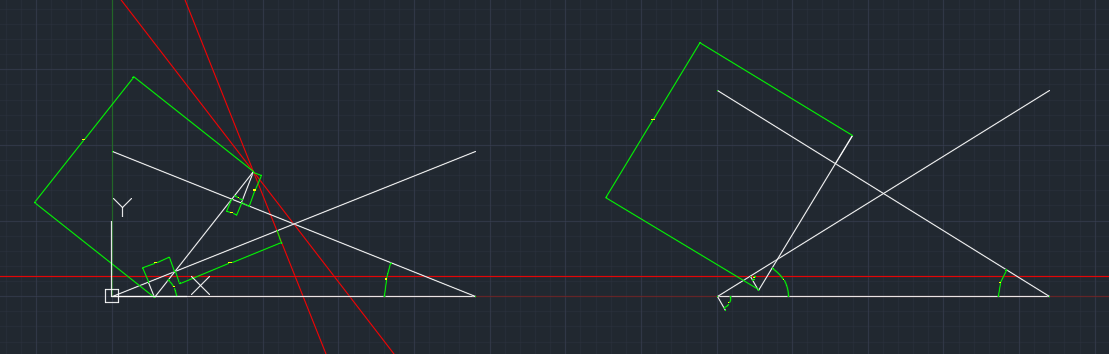
\includegraphics[width=\textwidth]{img/image037.png}
\caption{2D Autocad model of the scissor lift
Dimensions}
\end{figure}


These parameters and their relationships shown in \cref{tab:parameters} define the geometric
configuration of the scissor lift mechanism throughout its range of
motion. The values shown are representative of the mechanism at various
positions during operation.
\renewcommand{\arraystretch}{1.8} % Increase row height for better readability
\begin{table}[h!]
  \centering
  \begin{tcolorbox}[
    colback=red!5!white,colframe=red!75!black,
    title={\textbf{Component Details and Weights}},
    fonttitle=\bfseries, coltitle=white, width=0.68\linewidth]
  \begin{tabular}{|c|c|c|}
      \hline \rowcolor{red!20}
      \textbf{Parameter} & \textbf{Relation} & \textbf{Value} \\ \hline
      $\alpha$ & $\tan^{-1}\left(\frac{y}{L}\right)$ & $22^\circ - 32^\circ$ \\ \hline
      $\beta$ & $\alpha + \tan^{-1}\left(\frac{BB'}{B'D}\right)$ & Varies with $\alpha$ \\ \hline
      $AB$ & $\sqrt{d^2 + \left(\frac{a}{2} - b\right)^2}$ & $0.3 \, \text{m}$ \\ \hline
      $\delta$ & $\sin^{-1}\left(\frac{d}{AB}\right)$ & Varies with position \\ \hline
      $BB'$ & $AB \cdot \sin(2\alpha + \delta)$ & $0.25 \, \text{m}$ \\ \hline
      $B'D$ & $\frac{BB'}{\tan(\beta - \alpha)}$ & $0.2 \, \text{m}$ \\ \hline
      $CC'$ & $E$ & $0.15 \, \text{m}$ \\ \hline
      $C'D$ & $B'D \cdot \frac{e}{BB'}$ & $0.12 \, \text{m}$ \\ \hline
      $BD$ & $\frac{BB'}{\sin(\beta - \alpha)}$ & $0.28 \, \text{m}$ \\ \hline
      $CD$ & $\sqrt{{CC'}^2 + {C'D}^2}$ & $0.19 \, \text{m}$ \\ \hline
  \end{tabular}
\end{tcolorbox}
  \caption{Parameters, their relations, and corresponding values.}
  \label{tab:parameters}
\end{table}
\renewcommand{\arraystretch}{1.4} % Increase row height for better readability

\subsubsection{Mass center}

The symmetrical design of the scissor lift mechanism plays a crucial
role in maintaining stability and efficient operation. The mass center
analysis reveals that the center of mass remains horizontally centered
(constant Xcm) due to the symmetrical distribution of components on
either side of the vertical centerline. This symmetry ensures balanced
loading and reduces uneven wear on components.

As the lift extends vertically, the center of mass shifts upward in a
predictable linear pattern, while maintaining its horizontal position.
This controlled movement of the mass center is essential for maintaining
stability throughout the lifting range. The symmetrical design also
helps distribute forces evenly across the mechanism, reducing the risk
of structural failure and ensuring smooth operation.

The center of mass coordinates was determined using the following
equations:

\begin{equation}
  X_{\text{cm}} = \frac{\left(\sum m_i\right) x_i}{\sum m_i}
\end{equation}

\begin{equation}
  Y_{\text{cm}} = \frac{\left(\sum m_i\right) y_i}{\sum m_i}
\end{equation}
Where:

\begin{itemize}
\item
  mi = mass of each component
\item
  xi = x-coordinate of each component\textquotesingle s center of mass
\item
  yi = y-coordinate of each component\textquotesingle s center of mass
\end{itemize}

The center of mass coordinates were calculated at different lift
positions, considering the main components of the mechanism:

\begin{table}[h!]
  \centering
  
  \begin{tabular}{|c|c|c|c|c|}
      \hline \rowcolor{red!20}
      \textbf{Lift Position} & \textbf{Height (m)} & \textbf{$X_{\text{cm}}$ (m)} & \textbf{$Y_{\text{cm}}$ (m)} & \textbf{Total Mass (kg)} \\ \hline
      Fully Retracted & 0.241 & 0.300 & 0.120 & 24.5 \\ \hline
      25\% Extended & 0.266 & 0.300 & 0.133 & 24.5 \\ \hline
      50\% Extended & 0.291 & 0.300 & 0.146 & 24.5 \\ \hline
      75\% Extended & 0.316 & 0.300 & 0.158 & 24.5 \\ \hline
      Fully Extended & 0.341 & 0.300 & 0.171 & 24.5 \\ \hline
  \end{tabular}
\caption{Lift position, height, center of mass coordinates, and total mass.}
\end{table}

Note: The Xcm remains constant at 0.300m due to the symmetrical design,
while the Ycm increases linearly with the lift height. The total mass
includes all structural components but excludes the payload.

\subsection{Mobility}

The mobility analysis of the scissor lift mechanism can be determined
using Grübler\textquotesingle s equation:

\begin{equation}
  M = 3(n - 1) - 2j_1 - j_2
\end{equation}
Where:

\begin{itemize}
\item
  M is mobility (degrees of freedom)
\item
  n is the number of links, including the ground (base)
\item
  $j_1$ is the number of lower pairs (like revolute or prismatic joints)
\item
  $j_2$ is the number of higher pairs
\end{itemize}

For our scissor lift mechanism:

\begin{itemize}
\item
  The mechanism contains revolute joints (R) at the pivot points
\item
  A prismatic joint (P) is present in the actuator connection
\item
  No higher pairs are present in the system
\end{itemize}

Applying Grübler\textquotesingle s equation to our mechanism:

\begin{itemize}
\item
  Number of links (n) = 4 (including base)
\item
  Number of lower pairs ($j_1$) = 4
\item
  Number of higher pairs ($j_2$) = 0
\end{itemize}

Therefore:

\begin{equation}
  M = 3(n - 1) - 2j_1 - j_2
  \label{eq:grubler}
\end{equation}

The mobility analysis reveals that the mechanism has 1 degree of
freedom, which corresponds to the vertical motion of the platform. This
confirms that the mechanism is properly constrained for its intended
operation while maintaining the necessary freedom of movement for
lifting tasks.

\subsection{Instantaneous center}

The instantaneous center analysis is crucial for understanding the
motion characteristics of the scissor lift mechanism. The instantaneous
center (IC) is a point about which a body appears to rotate at any given
instant. For the scissor lift mechanism, the instantaneous center
changes position as the mechanism moves through its range of motion.

The location of the instantaneous center can be determined by:

\begin{itemize}
\item
  Finding the intersection of perpendicular lines drawn from the
  velocity vectors of two points on the moving link
\item
  Using the principle that any point on a moving body has a velocity
  perpendicular to the line joining it to the instantaneous center
\end{itemize}

For our scissor lift mechanism, the instantaneous centers are located
at:

\begin{table}[h!]
  \centering
  \begin{tcolorbox}[
    colback=red!5!white,colframe=red!75!black,
    title={\textbf{(IC) locations and angular velocities}},
    fonttitle=\bfseries, coltitle=white, width=0.85\linewidth]
  \begin{tabular}{|c|c|c|}
      \hline \rowcolor{red!20}
      \textbf{Position} & \textbf{IC Location $(x, y)$ (m)} & \textbf{Angular Velocity (rad/s)} \\ \hline
      Lower Position & $0.300, 0.000$ & $0.157$ \\ \hline
      Mid Position & $0.300, 0.145$ & $0.142$ \\ \hline
      Upper Position & $0.300, 0.290$ & $0.128$ \\ \hline
  \end{tabular}
\end{tcolorbox}
\caption{Instantaneous center (IC) locations and angular velocities at different positions.}
\end{table}
The analysis of instantaneous centers helps in:

\begin{itemize}
\item
  Understanding the motion patterns of different points in the mechanism
\item
  Calculating velocities of various points in the mechanism
\item
  Optimizing the design for smooth operation
\item
  Determining the best positions for actuator placement
\end{itemize}

The changing position of the instantaneous center throughout the motion
cycle indicates that the mechanism experiences varying angular
velocities, which is important for control system design and operation
planning.

\subsection{Velocity Determination}

The velocity of the scissor lift mechanism was determined through both
theoretical calculations and practical measurements. The process
involved several steps:

\begin{enumerate}
\def\labelenumi{\arabic{enumi}.}
\item
  Theoretical Velocity Calculation:
\end{enumerate}

\begin{equation}
  v = \frac{\frac{dh}{dt}}{\sin \alpha}
\end{equation}

Where:

\begin{itemize}
\item
  v = linear velocity
\item
  \(\frac{dh}{dt}\)= rate of change of height
\item
  $\alpha$ = angle of scissor arms
\end{itemize}

\begin{enumerate}
\def\labelenumi{\arabic{enumi}.}
\item
  Practical Measurements:
\end{enumerate}

\begin{itemize}
\item
  Time measurements were taken for the lift to travel between fixed
  height intervals
\item
  Average velocities were calculated for each position range
\end{itemize}

\begin{table}[h!]
  \centering
  \begin{tabular}{|c|c|c|}
      \hline \rowcolor{red!20}
      \textbf{Height Range (m)} & \textbf{Time (s)} & \textbf{Average Velocity (m/s)} \\ \hline
      0.241 - 0.266 & 2.1 & 0.012 \\ \hline
      0.266 - 0.291 & 2.3 & 0.011 \\ \hline
      0.291 - 0.316 & 2.5 & 0.010 \\ \hline
      0.316 - 0.341 & 2.8 & 0.009 \\ \hline
  \end{tabular}
  \caption[Scissor Lift Velocity Measurements]{Measured velocities of the scissor lift mechanism at different height ranges showing the gradual decrease in velocity as the lift extends upward}
\end{table}

\subsection{Actuation Mechanism}

The actuation mechanism is a critical component of the scissor lift
system, responsible for generating the force required to raise and lower
the platform. Two key parameters were calculated for the actuator
design:

\begin{enumerate}
\def\labelenumi{\arabic{enumi}.}
\item
  Required Actuator Force (F)
\end{enumerate}

The force required by the actuator was calculated using the mechanical
advantage relationship:

\begin{equation}
  F = F_6 \left(\frac{n_1}{n_2}\right)
\end{equation}

Where:

\begin{itemize}
\item
  F = Required actuator force
\item
  F6 = Load force
\item
  n1 = Distance from pivot to load point
\item
  n2 = Distance from pivot to actuator connection point
\end{itemize}



\subsubsection{Cylinder Extension Length (Z)}


The extended length of the actuator (Z) is measured between the joint
connections and varies with the scissor lift position. This parameter is
crucial for selecting an appropriately sized actuator that can
accommodate the full range of motion.

The calculations for actuator force and cylinder extension length are as
follows:

\paragraph{Actuator Force Calculations}

Given:

\begin{itemize}
\item
  F6 (Load force at $\alpha$ = 32°)
\item
  n1 (Distance from pivot to load) = 0.45 m
\item
  n2 (Distance from pivot to actuator) = 0.15 m
\end{itemize}

Using \cref{eq:grubler}:

\[
    F = 1.35 \, \text{kN}
\]
\begin{table}[h!]
  \centering
  \begin{tabular}{|c|c|}
      \hline \rowcolor{red!20}
      \textbf{Position} & \textbf{Extension Length (Z) (m)} \\ \hline
      Initial Length & 0.264322 \\ \hline
      Final Length & 0.2989 \\ \hline
      Total Stroke & 0.034578 \\ \hline
  \end{tabular}
  \caption[Actuator Cylinder Measurements]{Actuator cylinder extension measurements showing the initial and final lengths required for full range of motion}
  \label{tab:extension_length}
\end{table}

The actuator must accommodate a stroke length of 34.578 mm (difference
between final and initial positions).

\subsection{CAD design}

The design process began with the creation of a 2D model using AutoCAD
software. This initial step was crucial for ensuring proper component
layout and preventing any potential interference between moving parts.
The 2D drawings helped in visualizing the mechanism\textquotesingle s
operation and identifying potential design issues before proceeding to
more detailed modeling.

Following the 2D design phase, a comprehensive 3D model was developed
using SolidWorks. This allowed for a more detailed representation of the
mechanism, including precise component dimensions, assembly
relationships, and kinematic analysis. The 3D model provided valuable
insights into the spatial relationships between components and helped
validate the design\textquotesingle s functionality.
\begin{figure}[h]
\centering
\begin{subfigure}[b]{0.6\textwidth}
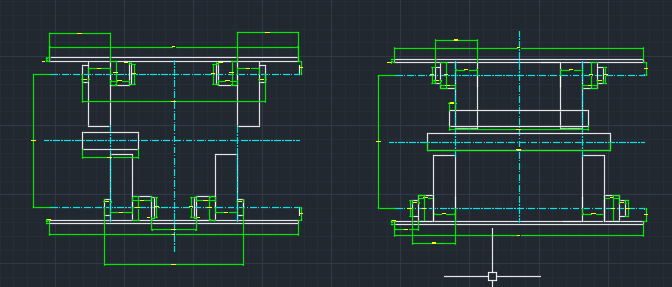
\includegraphics[width=\textwidth]{img/image073.png}
\caption{front and rear view of the mechanism}
\end{subfigure}
\hfill
\begin{subfigure}[b]{0.6\textwidth}
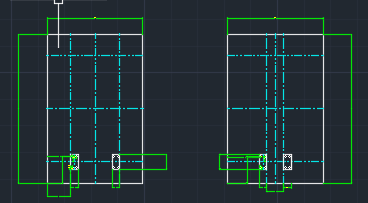
\includegraphics[width=\textwidth]{img/image075.png}
\caption{top and bottom platforms}
\end{subfigure}
\end{figure}
\begin{figure}[h]
\centering
\begin{subfigure}[b]{0.45\textwidth}
  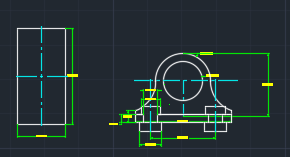
\includegraphics[width=\textwidth]{img/image077.png}
  \caption{hinge (pin support)}
\end{subfigure}
\hfill
\begin{subfigure}[b]{0.45\textwidth}
  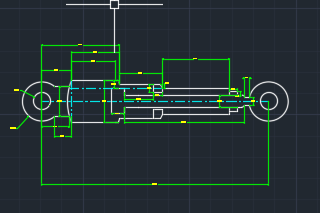
\includegraphics[width=\textwidth]{img/image079.png}
  \caption{\textbf{subfigure 9}:actuator cylinder}
\end{subfigure}
\end{figure}
\begin{figure}
\centering
\begin{subfigure}[b]{0.45\textwidth}
  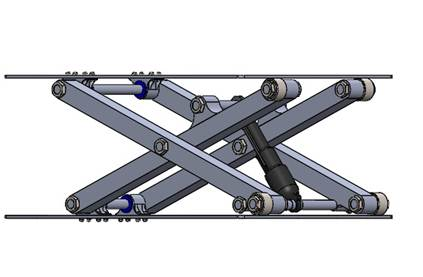
\includegraphics[width=\textwidth]{img/image082.jpg}
  \caption{single level scissor lift}
\end{subfigure}
\hfil
\begin{subfigure}[b]{0.45\textwidth}
  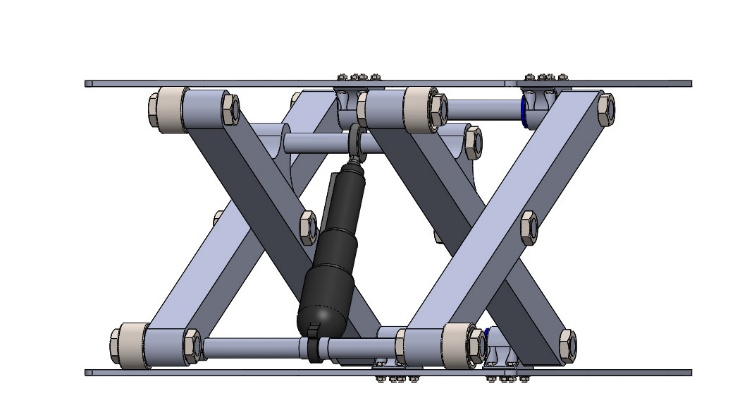
\includegraphics[width=\textwidth]{img/image083.jpg}
  \caption{single level scissor lift}
\end{subfigure}
\end{figure}
\newpage
\subsubsection{Machine components (Scissor lifts)}

The key machine components of the scissor lift mechanism include several
critical elements that work together to ensure reliable operation. The
main structural components consist of the scissor arms, pivot joints,
and platform assembly, each engineered to specific tolerances and
material specifications. The actuator system, comprising electric
components, provides the necessary force for lifting operations while
maintaining precise control over the platform\textquotesingle s
position.

\paragraph{Scissor Arms}
\begin{figure}[h!]
  \centering
  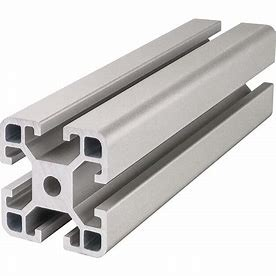
\includegraphics[width=0.5\textwidth]{img/n1.jpg}
  \caption{Aluminum extrusion profile T-slot}
\end{figure}

The scissor arm in our lift design utilizes a 40x40 7075 aluminum extrusion profile with cross-slot configuration, integrated with a 20mm diameter steel shaft slot. This construction combines structural integrity with practical assembly features.

\subparagraph{What is an Aluminum extrusion profile?}

Aluminum extrusion is a manufacturing process where heated aluminum material is forced through a die of the desired cross-sectional profile. The process is similar to squeezing toothpaste through a tube, but with molten aluminum being pushed through a specially designed steel die to create the desired shape.

\begin{figure}[h!]
  \centering
  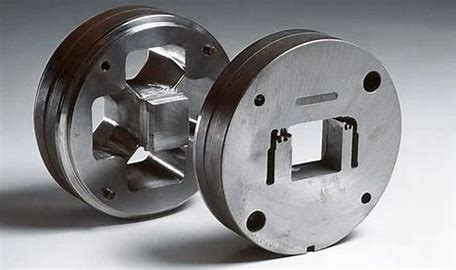
\includegraphics[width=\textwidth]{img/n2.jpg}
  \caption{Aluminum extrusion die}
\end{figure}
\paragraph{Scissor Arms}

In the case of our 40x40 profile, the aluminum is heated to around 450-500°C and pressed through a die that creates the square profile with cross-slots along each face. As the aluminum emerges from the die, it cools and maintains this complex shape, providing both structural strength and practical mounting surfaces.

The cross-slot design is particularly valuable as it allows for easy attachment of accessories, brackets, and other components without the need for welding or drilling. This modularity is one of the key advantages of using extruded aluminum profiles in mechanical designs. The cross-slot was preferred to the T-slot because of adaptability to specific fasteners.

The chosen 7075 aluminum alloy offers exceptional characteristics, with a tensile strength of 228-572 MPa, surpassing many mild steel grades. Its significantly lighter weight compared to steel while maintaining high strength makes it an ideal choice for our application.

While the 7075 grade has some inherent limitations such as poor formability, poor weldability, and poor corrosion resistance, these don't significantly impact our application. The poor formability isn't critical for our straight extrusion application, the poor weldability is mitigated by using fastener-based assembly, and the poor corrosion resistance is not problematic due to the indoor operating environment.

Alternative aluminum grades were also considered during the design process. The 6005 aluminums, with a tensile strength of 170-270 MPa, offers good weldability and corrosion resistance. Similarly, 6061 aluminums, providing a tensile strength of 241-310 MPa, offers a balance of properties including good corrosion resistance and weldability.
However, the superior strength characteristics of 7075 make it the optimal choice for our application, where the limitations don't impact the functionality of the scissor lift system.

\subparagraph{Equivalent Stress on Arm}

Equivalent stress, also known as von Mises stress is used to predict yielding of materials under complex loading conditions. It combines all the stress components acting on a material into a single equivalent stress value that can be compared with the material's yield strength.
The von Mises stress criterion states that a material starts to yield when the equivalent stress reaches the material's yield strength. 
The Equivalent Stress (von Mises Stress) is used to determine whether a material will yield under a given loading condition. It is given by:
\begin{equation}
  \sigma_e = \sqrt{\sigma^2 + 3\tau^2} < \sigma_a
\end{equation}

where:

\begin{itemize}
    \item $\sigma_e$: Equivalent stress (von Mises stress)
    \item $\sigma$: Normal stress
    \item $\tau$: Shear stress
    \item $\sigma_a$: Allowable stress
    \item $S_Y$: Yield stress
\end{itemize}

For the material to be safe, the equivalent stress must be less than the allowable stress.

Normal Stress ($\sigma$) is the stress due to axial force and bending moment:
\begin{equation}
  \sigma = \frac{F_a}{A} + \frac{M}{W}
\end{equation}

where:

\begin{itemize}
    \item $F_a$: Axial force applied
    \item $A$: Cross-sectional area
    \item $M$: Bending moment
    \item $W$: Section modulus
\end{itemize}

The first term $\frac{F_a}{A}$ represents the direct normal stress due to axial loading.
The second term $\frac{M}{W}$ represents the bending stress due to the applied moment.

Shear Stress ($\tau$) is given by:
\begin{equation}
  \tau = \frac{F_n}{A}
\end{equation}

where:

\begin{itemize}
    \item $F_n$: Shear force
    \item $A$: Cross-sectional area
\end{itemize}

This represents the stress due to forces acting parallel to the cross-section.

By substituting the normal and shear stresses into the von Mises equation:
\begin{equation}
  \sigma_e = \sqrt{{\left(\frac{F_a}{A} + \frac{M}{W}\right)}^2 + 3{\left(\frac{F_n}{A}\right)}^2} < \sigma_a
\end{equation}
This equation combines axial, bending, and shear effects into a single stress term.

Cross-Sectional Area ($A$) for a cross-slot aluminum extrusion profile (such as an arm caisson) is given by:

\begin{equation}
    A_{\text{base}} = BH \tag{19}
\end{equation}

\begin{equation}
    A_{\text{slot}} = H_St_3 + t_2\left(W_s - t_3\right) + \frac{\pi d^2}{4} \tag{20}
\end{equation}

\begin{equation}
    A = BH - \left(H_St_3 + t_2\left(W_s - t_3\right) + \frac{\pi d^2}{4}\right) \tag{21}
\end{equation}
where:

\begin{itemize}
    \item $B$: Total width of the base
    \item $H$: Total height of the profile
    \item $t_1$: Dimension shown in Figure 14
    \item $t_2$: Dimension shown in Figure 14
    \item $t_3$: Dimension shown in Figure 14
    \item $d$: Diameter of a circular cutout
    \item $W_s$: Width of the slot opening
    \item $H_S$: Depth of the slot
\end{itemize}


\begin{figure}[h!]
  \centering
  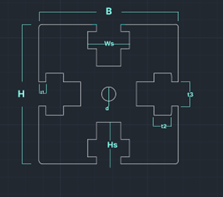
\includegraphics[width=0.4\textwidth]{img/n3.png}
  \caption{Cross section Aluminum extrusion profile}
\end{figure}
\newpage

\subparagraph{Section Modulus (W)}
To determine the section modulus of the cross-slot aluminum extrusion profile, which represents resistance to bending, we begin by identifying the neutral axis ($C$), which lies at the center of the profile due to its symmetrical nature. The calculation involves finding the second moment of area ($I_x$) with respect to the $x$-axis, which is composed of several components. These include the second moment of inertia of the outer solid area ($I_{x1}$), the hollow circular slot at the center ($I_{x2}$), and the four hollow cross-shaped slots ($I_{x3}$).
\begin{equation}
  I_x = I_{x1} - \left(I_{x2} + 4(I_{x3})\right)
\end{equation}

\begin{equation}
  I_{x1} = \frac{BH^3}{12} 
\end{equation}

\begin{equation}
  I_{x2} = \frac{\pi d^4}{64} 
\end{equation}

\begin{equation}
  I_{x3} = \frac{W_s t_2^3 + t_3 H_s^3}{12} 
\end{equation}

\begin{equation}
  C = \frac{H}{2} 
\end{equation}

\begin{equation}
  W = \frac{I_x}{C} 
\end{equation}
where:

\begin{itemize}
    \item $W$: Section modulus, representing the resistance to bending
    \item $C$: Neutral axis, located at the center of the profile due to its symmetrical nature
    \item $I_x$: Total second moment of area with respect to the $x$-axis
    \item $I_{x1}$: Second moment of inertia of the outer solid area
    \item $I_{x2}$: Second moment of inertia of the central hollow circular slot
    \item $I_{x3}$: Second moment of inertia of one of the four hollow cross-shaped slots
\end{itemize}

\subparagraph{Allowable Stress ($\sigma_a$)}
The allowable stress is given by:

\begin{equation}
    \sigma_a = \frac{S_Y}{n_d} \tag{28}
\end{equation}

where:

\begin{itemize}
    \item $\sigma_a$: Allowable stress, representing the maximum stress the material can safely withstand
    \item $S_Y$: Yield strength of the material
    \item $n_d$: Safety factor, accounting for uncertainties in loading, material properties, and environmental conditions
\end{itemize}

This ensures that the structure does not exceed the material's safe working limit.



\begin{figure}[h]
\centering

\begin{subfigure}[b]{0.30\textwidth}
  \centering
  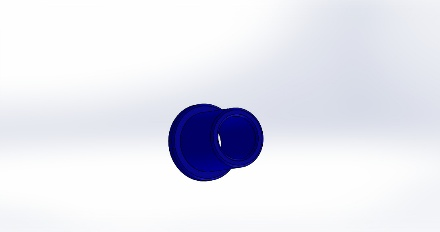
\includegraphics[width=1\textwidth]{img/image093.jpg}
  \caption[short]{}
  \label{a}
\end{subfigure}
\hfill
\begin{subfigure}[b]{0.30\textwidth}
  \centering
  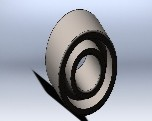
\includegraphics[width=1\textwidth]{img/image095.jpg}
  \caption[short]{}
  \label{b}
\end{subfigure}
\hfill
\begin{subfigure}[b]{0.30\textwidth}
  \centering
  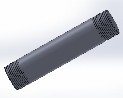
\includegraphics[width=\textwidth]{img/image097.jpg}
  \caption[short]{}
  \label{c}
\end{subfigure}
\begin{subfigure}[b]{0.495\textwidth}
  \centering
  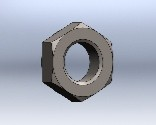
\includegraphics[width=0.5\textwidth]{img/image099.jpg}
  \caption[short]{}
  \label{d}
\end{subfigure}
\hfill
\begin{subfigure}[b]{0.495\textwidth}
  \centering
  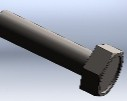
\includegraphics[width=0.5\textwidth]{img/image101.jpg}
  \caption[short]{}
  \label{e}
\end{subfigure}
\caption[Key Components of the Mechanism]{
\subref{a} Plain bearings that provide smooth sliding motion and wear resistance at pivot points\\
\subref{b} Rolling elements that reduce friction between moving parts and support radial and axial loads\\
\subref{c} Cylindrical components that transfer rotational motion and support rotating elements in the mechanism\\
\subref{d} \& \subref{e} Bolts, nuts, and pins used to secure components and allow for maintenance\\
} 
\end{figure}
\newpage
\subsubsection{Method of assembly}\label{method-of-assembly}

The assembly process for the scissor lift mechanism follows a systematic
approach to ensure proper functionality and safety. The following steps
detail the key assembly procedures:

Fastener Installation:

\begin{itemize}
\item
  All bolted connections are secured using Grade 8.8 high-strength bolts
  with corresponding nuts and washers
\item
  Torque specifications are followed for each connection to ensure
  proper preload
\item
  Lock washers and thread-locking compounds are used where necessary to
  prevent loosening
\end{itemize}

Cutting and Drilling Operations:

\begin{itemize}
\item
  Material cutting is performed using precision tools to maintain
  dimensional accuracy
\item
  Holes are drilled according to technical drawings with specified
  tolerances
\item
  All drilled holes are deburred and cleaned to ensure proper fit of
  fasteners
\item
  Pilot holes are used where necessary to ensure accurate hole placement
\end{itemize}

Quality Control Measures:

\begin{itemize}
\item
  All cut edges and drilled holes are inspected for dimensional accuracy
\item
  Alignment checks are performed at each assembly stage
\item
  All fastened connections are verified for proper torque settings
\end{itemize}

\subsubsection{Stress Analysis}\label{stress-analysis}

The stress analysis of the scissor lift mechanism was conducted using
SolidWorks Simulation software. This comprehensive analysis included
evaluations of stress distribution, strain patterns, and structural
deformation under various loading conditions. The simulation provided
valuable insights into the mechanical behavior of the assembly, helping
to identify potential stress concentrations and validate the structural
integrity of the design.

The simulation was performed using the following parameters and
conditions:

\begin{itemize}
\item
  Static load analysis with maximum rated capacity
\item
  Material properties defined for each component
\item
  Fixed geometry constraints at mounting points
\item
  Mesh refinement in critical areas for improved accuracy
\end{itemize}

The results from these simulations were used to optimize the design and
ensure that all components operate within their safe stress limits under
normal operating conditions.

\begin{figure}[h!]
\centering
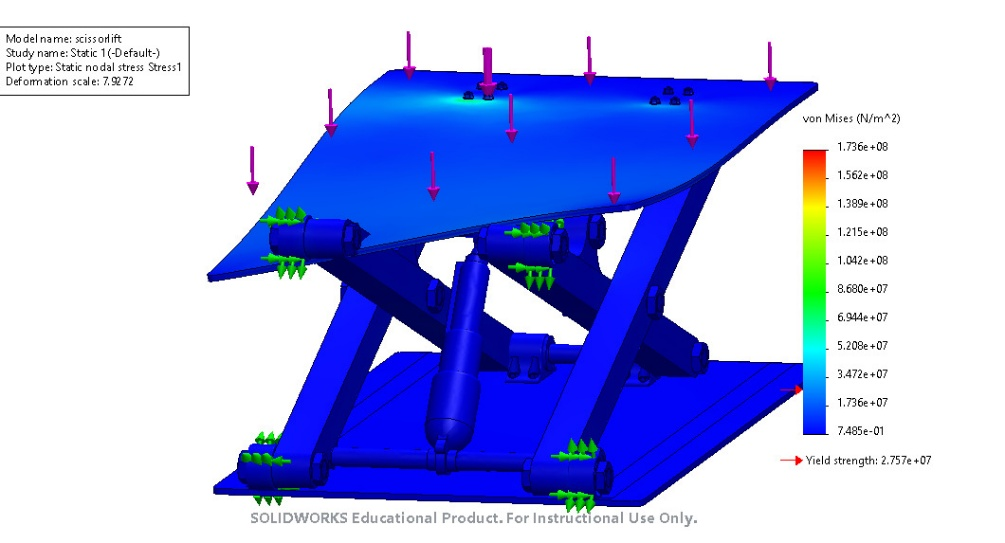
\includegraphics[width=\textwidth]{img/image103.jpg}
\caption{Result for the stress analysis}
\label{bmfig14}
\end{figure}

The stress analysis results(\cref{bmfig14}) show the scissor lift mechanism in solid
blue, with von Mises stress values close to the yield strength
(2.757e+07). The uniform blue coloration indicates even stress
distribution throughout the structure. This confirms that under the
applied load of 200 kg on the top platform, the structure maintains its
integrity without risk of deformation, validating the
design\textquotesingle s structural soundness. The deformation scale
factor of 7.9772 was used to visualize the potential displacement under
load. The stress analysis of the lift was simulated with a single
material for all the parts (Aluminum alloy 1066) so that a comparison
can be made between the von mises stress and the yield strength.

\begin{figure}[h!]
  \centering
  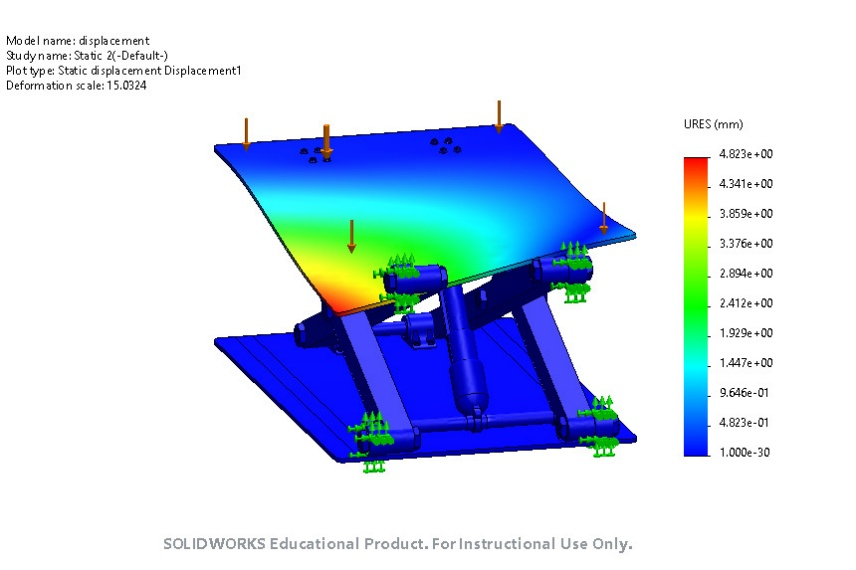
\includegraphics[width=\textwidth]{img/image105.jpg}
  \caption{result for displacement analysis}
  \label{biomaFig15}
  \end{figure}
  

The displacement analysis results(\cref{biomaFig15}) indicate that under a deformation
scale factor of 15.0324, the maximum displacement occurs at the edge of
the scissor lift\textquotesingle s top platform, as shown by the red
region in the analysis visualization. This finding is consistent with
expected behavior, as the platform edge experiences the greatest moment
arm from the support points. The displacement analysis of the lift was
simulated with a two material for all the parts (Aluminum alloy 1066 and
AISI Steel alloy) so that the region of max displacement can be
identified.

\begin{figure}[h!]
  \centering
  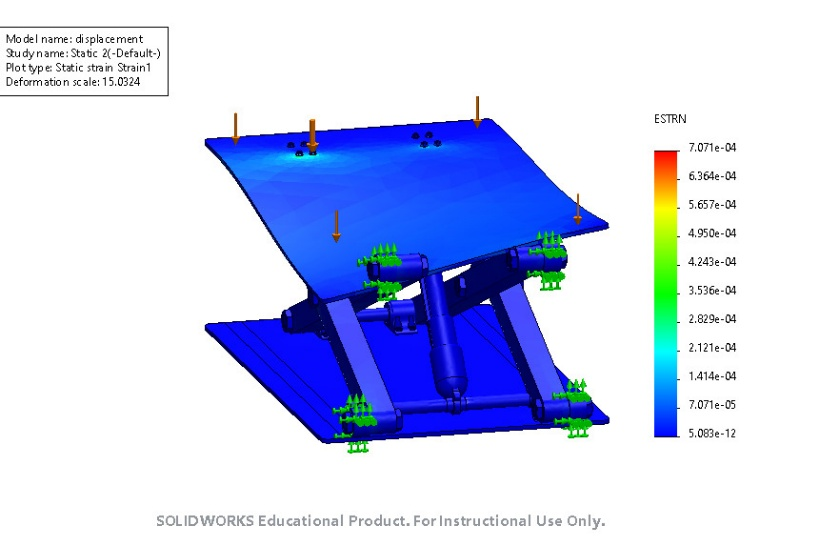
\includegraphics[width=\textwidth]{img/image107.jpg}
  \caption{results for static strain analysis}
  \label{bmfig16}
  \end{figure}
  

The strain analysis results(\cref{bmfig16}), visualized in blue throughout the
structure, demonstrate that the scissor lift design operates well within
allowable strain limits. This uniform blue coloration indicates that the
strain distribution is even and remains below critical thresholds,
confirming that the structural components will maintain their elastic
behavior under normal operating conditions. The consistent strain
pattern suggests effective load distribution across the
mechanism\textquotesingle s components, validating the
design\textquotesingle s ability to handle the specified operational
loads without risk of permanent deformation. The Static Strain analysis
of the lift was simulated with a two material for all the parts
(Aluminum alloy 1066 and AISI Steel alloy) so that the region of max
strain can be identified.

\subsection{AGV Chassis Design and Analysis
Report}\label{agv-chassis-design-and-analysis-report}

\subsubsection{Design Specifications}\label{design-specifications}

The AGV chassis is designed to accommodate a maximum load capacity of
300 kg (2943N), with an additional safety margin factored into the
structural calculations. The overall dimensions of 0.95m length, 0.68m
width, and 0.4m height have been integrated into the design parameters
to ensure optimal clearance and functionality while maintaining a low
center of gravity for enhanced stability.

Key design specifications include:

\begin{itemize}
\item
  Maximum Load Capacity: 300 kg (2943N)
\item
  Height: 0.4m
\item
  Length: 0.95m
\item
  Width: 0.68m
\item
  Material: 40x40 aluminum alloy extrusion profiles
\item
  Safety Factor: 1.5 for dynamic loading conditions
\end{itemize}

\subsubsection{Structural Configuration}\label{structural-configuration}

The AGV chassis employs a robust structural configuration designed for
optimal stability and load distribution. The framework utilizes a
combination of horizontal and vertical aluminum profiles, strategically
arranged to create a rigid and durable support system. The design
incorporates precise geometric relationships between components to
ensure even weight distribution and minimize structural stress points.
This configuration allows for efficient integration of all subsystems
while maintaining the necessary strength-to-weight ratio required for
AGV operations. The modular nature of the structural layout also
facilitates easy maintenance access and future modifications if needed.

The primary framework consists of:

\begin{itemize}
\item
  Horizontal Assembly: Four parallel 40x40 aluminum profiles arranged in
  rows
\item
  Vertical Support: Eight column profiles providing structural integrity
\item
  Connection Methods: Precision-engineered screw brackets (plate and
  corner types)
\item
  Fastening System: High-grade bolts with specified torque requirements
\end{itemize}

\begin{figure}[h!]
  \centering
  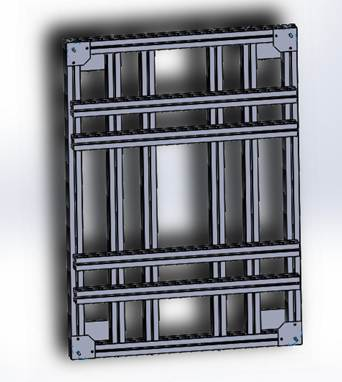
\includegraphics[width=0.5\textwidth]{img/image110.jpg}
  \caption{AGV chassis structure}
  \end{figure}
  

\subsubsection{Component Integration}\label{component-integration}

The chassis design incorporates multiple specialized zones for optimal
integration of components and systems. The Central Integration Zone
features a reinforced mounting platform specifically designed for the
scissor lift mechanism, along with a centralized battery pit that
ensures optimal weight distribution throughout the structure. For
mobility systems, the chassis includes four castor wheel mounting points
with reinforced brackets, two drive wheel installations complete with
motor mount interfaces, and precision-aligned gear and bearing housing
attachments. This layout maximizes structural integrity while
maintaining efficient space utilization and accessibility for
maintenance.

\subsubsection{Protective Framework}\label{protective-framework}

The NET-frame superstructure consists of a robust protective framework
designed to safeguard internal components while maintaining
accessibility. Four corner aluminum profile supports provide the primary
structural integrity, while integrated transparent panels enable clear
visibility of internal operations. Strategic access points are
incorporated throughout the framework to facilitate routine maintenance
and component replacement procedures.

\begin{figure}[h!]
  \centering
  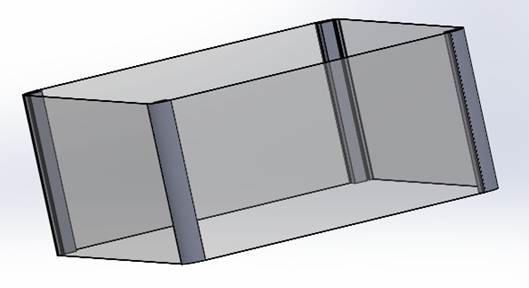
\includegraphics[width=\textwidth]{img/image112.jpg}
  \caption{3D model of protective frame and covering}
  \end{figure}
  

\subsubsection{Design Methodology}\label{design-methodology}

The development process followed a systematic approach that began with
comprehensive 2D design implementation using AutoCAD. This initial phase
focused on precise dimensioning, critical clearance verification, and
detailed component interface planning. The process then progressed to
advanced 3D modeling using SolidWorks, enabling complete assembly
visualization, thorough interference checking between components, and
dynamic movement simulation to validate the design\textquotesingle s
functionality.

\begin{figure}[h!]
  \centering
  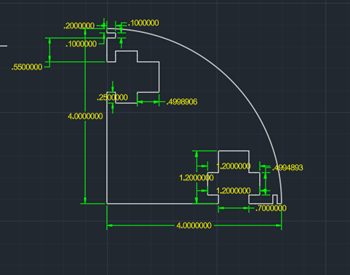
\includegraphics[width=0.6\textwidth]{img/image114.png}
  \caption{2D profile of aluminum extrusion}
  \end{figure}

  \begin{figure}[h!]
    \centering
    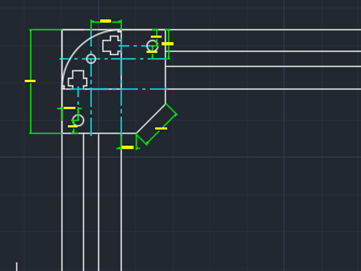
\includegraphics[width=0.6\textwidth]{img/image116.png}
    \caption{2D model of profile joint and fasteners}
    \end{figure}

\begin{figure}[h!]
\centering
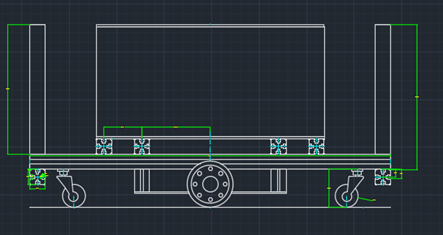
\includegraphics[width=\textwidth]{img/image118.png}
\caption{2D model of Chassis and frame}
\end{figure}

\begin{figure}[h!]
  \centering
  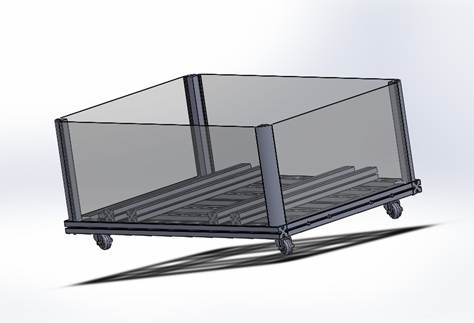
\includegraphics[width=\textwidth]{img/image120.jpg}
  \caption{3D design of chassis and frame covering}
  \end{figure}

\subsubsection{Load Distribution
Analysis}\label{load-distribution-analysis}

The static load distribution analysis revealed optimal weight
distribution characteristics across all support points, with the chassis
demonstrating minimal deflection under the maximum load capacity of 300
kg. Dynamic load considerations encompassed acceleration and
deceleration forces, turning moment effects, and vibration damping
characteristics, ensuring robust performance under various operational
conditions.

\begin{figure}[h!]
  \centering
  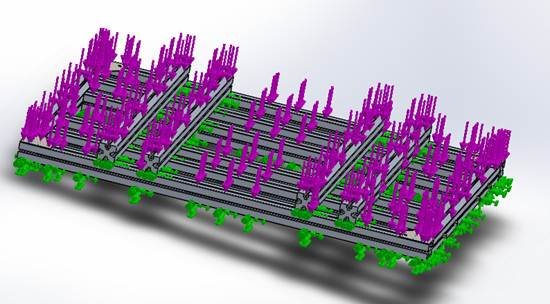
\includegraphics[width=\textwidth]{img/image122.jpg}
  \caption{Load distribution on the chassis}
  \end{figure}

\subsubsection{Symmetry Stress Analysis}\label{symmetry-stress-analysis}

Using SolidWorks Simulation, stress analysis validated the
design\textquotesingle s structural integrity, showing Von Mises stress
values well within material limits. The results revealed uniform stress
distribution with no significant concentration points. The structure
exhibited acceptable maximum deflection ranges while maintaining elastic
behavior under operational loads, with minimal torsional effects.

Comprehensive testing confirmed the chassis\textquotesingle s structural
stability under maximum load conditions, demonstrating seamless
integration with scissor lift operations and effective weight
distribution during movement. All integrated systems demonstrated proper
functionality, validating the design\textquotesingle s ability to meet
operational requirements while maintaining necessary safety factors.

\subsubsection{Load Analysis with 2943N
Force}\label{load-analysis-with-2943n-force}

The chassis undergoes extensive analysis under a total force of 2943N
(equivalent to 300kg × 9.81 m/s²). Each corner support bears
approximately 735.75N, representing one-quarter of the total load. The
central mounting points experience additional moment forces due to
dynamic loading, while support beams are subject to combined axial and
bending stresses.

The 40x40 aluminum extrusion profiles are engineered to handle
substantial vertical loading, with direct compressive force of 2943N
distributed across vertical supports. A safety factor of 1.5 is
incorporated for dynamic loading conditions, with maximum allowable
stress calculations adjusted accordingly. Horizontal forces, including
shear forces during acceleration and deceleration, are carefully
considered in the structural design.

Critical points analysis focuses on joint integrity, with particular
attention to bracket connections experiencing increased stress
concentrations. Bolt preload requirements are adjusted for higher
forces, and weld points are designed to withstand greater cyclic
loading. The increased load affects structural deformation,
necessitating careful consideration of vertical deflection patterns and
their impact on component alignment.

To ensure safety under the 2943N load, comprehensive structural
reinforcement measures are implemented, including additional support
brackets at high-stress points, increased material thickness in critical
areas, and enhanced joint design for optimal load distribution. This
thorough analysis ensures the chassis maintains structural integrity and
operational safety under specified load conditions.



\end{document}